\documentclass[UTF8,a4paper,11pt,oneside]{ctexbook}
\usepackage{amsmath,amssymb,amsfonts}
\usepackage{graphfig}
\usepackage{tikz}
\usepackage{graphicx}
\usepackage{anyfontsize}
\usepackage{circuitikz}
\usepackage{multirow}
\usepackage{geometry}
\usepackage[toc]{multitoc}
\usepackage[colorlinks]{hyperref}
\usetikzlibrary{calc}
\usetikzlibrary{math}
\geometry{a4paper,left=2.5cm,right=2.5cm,top=3cm,bottom=3cm}
\setlength{\headheight}{12.64723pt}
\addtolength{\topmargin}{-0.64723pt}
\setcounter{tocdepth}{1}
\linespread{1.8}\selectfont
\title{大气物理学}
\author{Cls\thanks{\href{https://github.com/Clignniis}{点击进入资料的github仓库}}}
\date{期末复习资料}
\begin{document}

\frontmatter 
\maketitle

大气物理学考试主要靠背,可能需要各位同学寻找其它相关资料。

因技术原因无法精确画出湿绝热线,此图片仅示意大致走向,具体求解请参考其他图片。

\tableofcontents

\mainmatter

\chapter{地球大气}

\section{地球大气演化的三个阶段}
\begin{enumerate}
    \item 原始大气(\(\mathrm{H}_2\)--\(\mathrm{He}\)型大气)
    \item 第二代大气(还原型大气)
    \item 现代大气(氧化型大气)
\end{enumerate}

\section{大气组成}
\begin{enumerate}
    \item 地球大气是由多种气体以及漂浮于其中的固态,液态等颗粒物质组成的,
    \item 干洁大气:不含水汽和悬浮颗粒物的大气称为干洁大气,
    \item 相变特征:在地球大气温压条件下,水汽是唯一能发生相变的气体成分,
    \item 空气密度:标准状态下,干空气密度为1.29\(\mathrm{kg\cdot{}m}^{-3}\),
    \item 平均分子量:90km以下,空气平均分子量为28.966,不随高度变化,90km以上,随高度递减。
\end{enumerate}

\section{大气气溶胶}

\subsection{气溶胶}

气溶胶是指悬浮在气体中的固体和(或)液体微粒与气体载体共同组成的多相体系。

\subsection{大气气溶胶}

大气气溶胶是指大气与悬浮在其中的固体和液体微粒共同组成的多相体系。

\subsection{气溶胶粒子}

PM10,又称为可吸入颗粒物(Inhalable Particles,IP),指粒径\(D_p\leq10\mathrm{\mu{}m}\)的颗粒物质量浓度。PM2.5,即细粒子,指粒径\(D_p\leq{}2.5\mathrm{\mu{}m}\)的颗粒物质量浓度。

\subsection{气溶胶来源}

气溶胶粒子的来源非常广泛,有天然源和人为源两种。
\begin{enumerate}
    \item 天然源:地球表面的岩石和土壤风化,海浪溅沫和海洋中的气泡炸裂形成的海盐粒子,植物花粉,孢子,火山爆发,森林火灾等。
    \item 人为源:农业活动,交通运输以及工业过程等各种人类活动。
\end{enumerate}

\subsection{气溶胶分类}

由排放源直接排放到大气中的颗粒物称为一次气溶胶,大气中的气体经光化学氧化或其他化学反应生成的颗粒物(即气--粒转化过程)称为二次气溶胶。

\subsection{气溶胶的去除}

气溶胶的汇是指气溶胶粒子的去除,包括干沉降和湿沉降。
\begin{enumerate}
    \item 干沉降是指气溶胶粒子在重力作用下或与地面其他物体碰撞后,发生沉降而被去除。
    \item 湿沉降过程:指质粒受雨雪或云雾等影响而下沉到下垫面移出大气的过程。包括凝长下沉,碰并下沉。(云内清除和云下清除)
\end{enumerate}

\section{大气分层}

依据温度随高度分布的特点,1962年世界气象组织根据中纬度气温铅直分布的平均状况,将大气分成:对流层,平流层,中间层和热层。

为了描述气温铅直分布特点,引入气温垂直递减率(简称气温直减率),表达式为:\(\gamma=-\dfrac{\partial{}T}{\partial{}z}\)
\subsection{对流层}
\begin{enumerate}
    \item 对流层(troposphere)位于大气最底部,其厚度在高纬地区平均约8--9km,中纬度地区平均约10--12km,低纬度地区平均17--18km,夏季厚度大于冬季。从地面到1--2km高度为行星边界层,其中的50--100m以下的气层称为近地层,近地层以上到边界层顶称为上部摩擦层。行星边界层以上的大气称为自由大气,在自由大气中,地表摩擦作用可忽略不计。对流层与平流层之间的过渡层,称为对流层顶,厚度约数百米到1--2km,对流展顶内的气温几乎不随高度变化。
    \item 对流层集中了约75%的大气和90%以上的水汽质量。
    \item 气温随高度增高而降低,北半球低纬地区平均气温直减率约\(6.5^\circ\mathrm{C\cdot{}km}^{-1}\)。
    \item 垂直运动剧烈,有利于大气成分在垂直方向上的输送。
    \item 主要天气现象都在对流层内形成。空气受地表影响很大,气象要素水平分布不均匀。
\end{enumerate}

\subsection{平流层}
\begin{enumerate}
    \item 自对流层顶向上到55km左右的气层为平流层(stratosphere),其上界称为平流层顶,此层约占有20%的大气质量。平流层内,温度从对流层顶到20km处几乎不随高度变化(1902年发现),再往上温度升高很快,到顶部可达\(-3\)~\(-7^\circ\mathrm{C}\)。
    \item 温度随高度升高,大气层结稳定。
    \item 空气垂直对流弱,以平流为主。
    \item 空气稀薄,能见度好,很少出现天气现象。
    \item 在15--35km范围内,有厚约20km的臭氧层。
\end{enumerate}

\subsection{中间层}
\begin{enumerate}
    \item 中间层(mesosphere)是指平流层顶到90km高度左右的大气层,其上界称为中间层顶。
    \item 气温随高度升高而降低,顶部温度可降至约\(-101^\circ\mathrm{C}\),是大气层最冷的部分。
    \item 垂直温度梯度大,有强烈的垂直混合,气压和密度随高度升高而降低的程度远小于低层大气。
    \item 水汽极少,几乎无云层。
\end{enumerate}

\subsection{热层}
\begin{enumerate}
    \item 中间层顶以上为热层,质量约占大气质量的十万分之一。热层中气体分子或原子很少发生碰撞。
    \item 热层温度随高度增加而迅速升高,由于分子氧和原子氧吸收紫外辐射,以及原子氧发生电离释放热量,因此温度可达1000K以上
    \item 热层温度变化与太阳活动有关,上层温度变化范围约500--\(2000^\circ\mathrm{C}\)。
    \item 热层没有明显的顶部,通常认为温度从增温转为等温时,即为热层顶部,其高度变化约在260--500km之间。
    \item 在这一层高纬度地区常出现极光现象。
\end{enumerate}

\chapter{气象要素的计算}

\section{气温与温标}

\subsection{热力学温标}

表示空气冷热程度的物理量,用以下几种温标来表示。
\begin{enumerate}
    \item 绝对温度(\(\mathrm{K}\))
    \item 华氏温度(\(^\circ\mathrm{F}\))
    \item 摄氏温度(\(^\circ\mathrm{C}\))
\end{enumerate}

三种温标之间的\textbf{转换}关系:\(\mathrm{K}={}^\circ\mathrm{C}+273.15,\quad^\circ\mathrm{C}=\dfrac{5}{9}(^\circ\mathrm{F}-32)\)

\subsection{温度带}

在寒冷无风的夜晚,冷空气沉淀在山谷,造成谷底较斜坡冷的情形。在中纬度比较暖的斜坡区称之为“温度带”(thermal belts),可避免农作物遭霜害或冻伤。

\section{空气湿度}

\subsection{定义}

表示空气中水汽含量多少或潮湿程度的物理量。

常见的湿度变量

绝对湿度(Absolute Humidity)
\begin{equation}
p=\dfrac{m_v}{V}(\mathrm{kg\cdot{}m}^{-3})
\end{equation}

比湿(Specific Humidity)
\begin{equation}
q=\dfrac{m_v}{m}(\mathrm{kg\cdot{}m}^{-1})
\end{equation}

混合比(Mixing Ratio)
\begin{equation}
r=w=\dfrac{m_v}{m_d}(\mathrm{kg\cdot{}m}^{-1})
\end{equation}

\subsection{水汽压与饱和水汽压}

空气中水汽含量也可以用从蒸发出来的水汽压强来描述。

\subsubsection{水汽压}

是指空气中水汽的分压强。总压强等于各个气体的压强之和(这种现象被称为道尔顿分压定律)。当空气块中水汽增加,则实际水汽压(\(e\))增大,所以实际水汽压可以很好地描述空气中水汽的总含量。但水汽压不能无限制地增加,在一定的温度下,如果水汽压增大到某一个极限值,空气中水汽就达到饱和,如果超过这个极限值,将会有一部分水汽凝结成液体水,这一极限值称为该温度下的饱和水汽压。

相对于纯水(冰)平面的饱和水汽压\(e_{sw}\)(\(e_{si}\))是温度的函数,随温度升高而增大,即已知温度\(T\)就可计算出饱和水汽压\(e_s\)。

\subsubsection{饱和混合比}

相对于水的饱和混合比\(w_s\),是指相对于纯水平面饱和的,给定体积空气内的水汽质量\(m_{vs}\),与干空气质量\(m_d\)之比,也就是
\begin{equation}
w_s=\dfrac{m_{vs}}{m_d}
\end{equation}

\subsubsection{相对湿度}

相对度(RH)是实际空气中的水蒸气量与在特定温度(和压力)下饱和所需的最大水蒸气量之比。它是空气的水蒸气含量与其容量的比值,因此
\begin{equation}
\mathrm{RH}=\dfrac{r}{r_s}\times100\%\approx\dfrac{e}{e_s}\times100\%
\end{equation}

\subsubsection{露点和霜点}
\begin{enumerate}
    \item 露点温度(dew point Td)是一定质量湿空气等压降温达到饱和时的温度。具体地,对于一定质量的空气,若令其等压冷却,则\(q\),\(r\)和\(e\)都将保持不变,饱和水汽压\(e_s\)却因温度的降低而减小。当\(e_s=e\)时,空气相对平水面达到饱和,这时对应的温度称为露点温度。显然,在露点温度时的饱和水汽压等于实际水汽压:\(e_s(T_d)=e\)
\end{enumerate}
\begin{figure}[htbp]
    \centering
\begin{tikzpicture}[>=latex]
    \draw[->] (0,0)--(0,5)node[right]{\(e\)};
    \draw[->] (0,0)--(5,0)node[right]{\(T\)};
    \node at(-0.2,-0.2){\(O\)};
    \foreach \x/\n in {1/\(T_d\),2/\(T_f\),3/\(T_o\),4/\(T_i\)}
    {
        \draw[dotted](\x,0)node[below]{\n}--(\x,\x*\x/4+1);
    }
    \foreach \y/\m in {1.25/\(e_i\),3.25/\(e_o\)}
    {
        \draw[dotted](0,\y)node[left]{\m}--(4,\y);
    }
    \draw [domain=1:4,samples=1000]
    plot(\x,{0.25*\x*\x+1});
    \draw[dashed](2,1.25)--(3,3.25)node[right]{\(O\)};
    \node at(1.2,1){\(D\)};
    \node at(2.2,1){\(F\)};
    \node at(4.2,1){\(M\)};
\end{tikzpicture}
    \caption{露点和霜点}
\end{figure}

\subsection{大气压强}

定义:气象科学上的大气压,是指单位面积上所受大气柱的重量(大气压强),也就是大气柱在单位面积上所施加的压力。
\begin{gather}
    1000\mathrm{hPa}=1000\mathrm{mb}=1\mathrm{bar}\\
    1013.25\mathrm{hPa}=76\mathrm{cmHg}
\end{gather}

\section{状态方程}

\subsection{理想气体状态方程}

在自然条件下,大气可看做理想气体,服从以下定律:
\begin{enumerate}
    \item 道尔顿分压定律\(p=\sum{}p_i\)
    \item 理想气体状态方程\(pV=\dfrac{m}{M}R^*T\)
    \item 即\(p=\rho{}RT\quad{}p\alpha=RT\quad{}\alpha=1/\rho\)
\end{enumerate}

\subsection{干空气状态方程}
\begin{equation}
p_d=\rho_dRT\quad{}\text{or}\quad{}p_d\alpha=R_dT
\end{equation}

\subsection{湿空气状态方程}

湿空气是由水汽和干空气混合组成。

湿空气的气压为:
\begin{equation}
    p=p_d+e
\end{equation}

湿空气的平均分子量:
\begin{equation}
    \overline{M}=\dfrac{m_d+m_v}{m_d/M_d+m_v/M_v}
\end{equation}

用混合比\(w\)表示上式,则:
\begin{equation}
    \overline{M}=\dfrac{1+w}{1/M_d+w/M_v}
\end{equation}

设:\(\varepsilon=M_v/M_d=0.622\),且\(w=q/(1-q)\),则上式改写为
\begin{equation}
M=M_d\dfrac{1+w}{1+w/\varepsilon}=M_d\dfrac{1}{1+(\dfrac{1}{\varepsilon}-1)q}=M_d\dfrac{1}{1+0.61q}
\end{equation}

因此,可得湿空气状态方程为
\begin{gather}
    p\alpha=R_{moist}T=\dfrac{R^*}{M}T=\dfrac{R^*}{M_d}(1+0.61q)T\\
    p\alpha=R_d(1+0.61q)T
\end{gather}

通过上式,定义一个新的变量--虚温:
\begin{equation}
    T_v=(1+0.61q)T
\end{equation}

虚温可以看作是考虑水汽后的订正温度。

虚温的物理意义:在相同气压的条件下,具有和湿空气相等的密度时的干空气所具有的温度。

注:虚温不可以直接被测量。虚温\(T_v\)与实际温度\(T\)之差叫虚温差\(\Delta{}T_v\)
\begin{equation}
\Delta{}T_v=T_v-T=0.61q\,T=0.378e/p\,T
\end{equation}

上式表示空气温度越高,水汽越多,虚温订正量越大。

\section{湿度变量之间的关系}

在实际大气中,混合比和比湿在数值上都是极小量(\(q,w\ll 1\)),且\(e\)远小于\(p\),所以可认为
\begin{equation}
w\approx{}q\approx\dfrac{\varepsilon{}e}{p}
\end{equation}

\section{比热}

混合气体的比热容为\(c\)

干空气的定压比热和定容比热分别为\(c_{pd}=1004\mathrm{J\cdot{}kg^{-1}\cdot{}K^{-1}}\)和\(c_{vd}=717\mathrm{J\cdot{}kg^{}\cdot{}K^{-1}}\)

湿空气的定压比热为\(c_p=\dfrac{m_dc_{pd}+m_vc_{pv}}{m_d+m_v}=c_{pd}(1+0.86q)\)

湿空气的定容比热为\(c_v=c_{vd}(1+0.96q)\)

\section{重力位势}

重力位势表示单位质量通过任意路径从海平面上升到某一高度\(z\)时克服重力所做的功,以\(\mathrm{J\cdot{}kg^{-1}}\)为单位,表达式为
\begin{equation}
\Phi=\int_0^zg\mathrm{d}\approx{}gz
\end{equation}

由于\(g\)是纬度和高度的函数,所以等位势面和等高面木同,它们彼此不平行。

两个等位势面之间的几何距离,赤道的大于极地,高空的大于低空。因等位势面上无重力分量,故沿着等位势面移动的物体不抵抗重力做功

\section{位势高度}

\subsection{定义}

气象上,习惯以位势高度\(Z\)表示位势的大小,单位是位势米(gpm)。它的定义式为
\begin{equation}
Z=\dfrac{\Phi}{g_0}=\dfrac{1}{g_0}\int_0^zg\mathrm{d}z=\dfrac{\bar{g}}{g_0}z
\end{equation}

\(g_0\)从物理意义上看,它是两种单位的换算因子,即
\begin{equation}
g_0=9.80665\mathrm{J\cdot{}kg^{-1}\cdot{}gpm^{-1}}
\end{equation}

1gpm相当于9.80665\(\mathrm{J\cdot{}kg^{-1}}\)的重力位势,即对单位质量空气克服地球引力做9.8J的功,则向上移动的高度为1gpm。

\subsection{应用}

气象上使用位势高度有很多优势,即:
\begin{enumerate}
    \item 可以不考虑重力加速度随高度和纬度的变化,根据实测的气压和温度即可计算位势高度,比较方便,
    \item 便于在理论上处理一些问题。例如在讨论大气能量时,垂直坐标若采用位势高度\(Z_g\),则重力无水平分量,方程得以简化。
\end{enumerate}

\chapter{大气方程}

\section{大气静力学方程}

\subsection{静力平衡}

实际大气在任何时候都处于运动状态,但是一般情况下空气的垂直加速度不超过\(10^{-3}\mathrm{m/s^2}\),远小于重力加速度,所以在垂直方向上,可将大气看成处于流体静力平衡状态,有强对流的地区除外。
\begin{equation}
\dfrac{\mathrm{d}p}{\mathrm{d}z}=-\rho{}g\quad\text{或}\quad\mathrm{d}p=-g\rho\mathrm{d}z
\end{equation}

上式即为静力学方程的一般形式。

\subsection{静力平衡条件下气压随高度分布有以下特点}
\begin{enumerate}
    \item 气压随高度增加而降低,即\(\mathrm{d}z>0\)时,\(\mathrm{d}p<0\),
    \item 若视\(g\)为常数,则\(p\)随\(z\)而减小的快慢程度主要取决于密度\(\rho\)
    \item 在静力平衡情况下,任意高度\(z\)处的大气压等于该高度单位截面上所承受的铅直空气柱的重量,即大气压的静力学意义:\(p=\int_z^\infty\rho{}g\mathrm{d}z\)据位势高度定义式\(\mathrm{d}\Phi=g\mathrm{d}Z=g_0\mathrm{d}z\)可得等价的大气静力学方程\(\mathrm{d}p=-\rho\mathrm{d}\Phi=-\rho{}g_0\mathrm{d}Z\)
\end{enumerate}

\subsection{大气的垂直温度梯度或温度垂直递减率(简称减温率)}
\begin{equation}
\Gamma=-\dfrac{\mathrm{d}T_v}{\mathrm{d}z}
\end{equation}

三种模式大气的垂直减温率分别为

等温大气:\(\Gamma=0\)

均质大气:\(\Gamma=34.2^\circ\mathrm{C\cdot{}km^{-1}}\)

多元大气:\(\Gamma=constant\)

\section{热力学过程--准静态过程}

当封闭系统状态变化过程进行地无限缓慢时,系统在变化过程中的每一步都处于平衡状态,称为准静态过程。系统在准静态过程中满足准静力条件,环境大气处于静力平衡状态

即
\begin{equation}
p\equiv{}p_e\quad\text{和}\quad\dfrac{\mathrm{d}p}{\mathrm{d}z}=\dfrac{\partial{}p_e}{\partial{}z}
\end{equation}

\section{热力学过程--绝热过程}

系统与外界只通过做功的方式互相作用,也就是说不通过热交换的方式,使系统的能量(能量是系统的态函数)发生变化的过程,称为绝热过程。

系统与外界只通过热交换或同时存在着做功的方式互相作用,使系统的能量发生变化的过程,称为非绝热过程。在非绝热过程中,系统与外界之间不一定有质量交换,例如在热传导过程中有能量交换而不发生质量交换,但也可以发生质量交换而使系统的能量发生改变。

\section{热力学过程--可逆过程}
一个过程,每一步都可在相反的方向进行而不在外界引起其他变化的,称为可逆过程。一般而言,如果过程进行的驱动力(如气体膨胀时内外压力差,热传导时的温度差等)无穷小,摩擦力(或耗散效应)无穷小,就可以看成可逆过程。可逆过程是研究平衡态性质的手段。

\chapter{热力学过程}

\section{干绝热过程}

\subsection{干绝热过程定义}

在绝热过程中,假设讨论对象是干空气,或者是无凝结,不含液态(固态)水的湿空气(即未饱和湿空气),这样的过程称之为干绝热过程。

干绝热减温率
\begin{equation}
\gamma_d=9.8\mathrm{K\cdot{}m^{-1}}
\end{equation}

\subsection{位温}

若要比较两个不同气块的温度,不能直接根据气块的温度变化来判断热量收支,也不能依据不同气压条件下的气温来比较不同气块的冷暖性质,必须将两个气块移至同一高度下才能互相比较其温度高低。为了建立温度比较的标准,在大气科学研究中提出了一个重要的温度度量参数--位温

对于干空气,位温定义为:干空气块从当前状态按照干绝热过程膨胀或者压缩到标准气压1000hPa时应该具有的温度,即
\begin{equation}
\theta=T\left(\dfrac{1000}{p}\right)^{k_d}
\end{equation}

在干绝热过程中\(\mathrm{d}Q=0\),所以\(\mathrm{d}\theta=0\),即干绝热过程中位温\(\theta\)是守恒量。

若某一层大气的减温率\(\Gamma=\gamma_d\),则整层大气位温必然相等。在对流层内,一般情况下大气垂直减温率\(\Gamma<\gamma_d\),所以有\(\dfrac{\mathrm{d}\theta}{\mathrm{d}z}>0\),表明位温随高度增加而增加。

\subsection{抬升凝结高度}
未饱和湿空气块干绝热上升刚好达到饱和的高度,称为抬升凝结高度(Lifting Condensation Level,LCL)。在LCL高度处的气压和温度分别称为饱和气压\(p_c\)和饱和温度\(T_c\)。

\section{湿绝热过程}

\subsection{可逆饱和绝热过程(可逆湿绝热):有云无降水}

水汽相变所产生的水成物不脱离原气块,始终跟随气块上升或下降,所释放的潜热也全部保留在气块内部。可逆湿绝热过程中\(L\)和\(m_d\)都是保守开放系统。

\subsection{假绝热过程:全部为降水但无云}

水汽相变产生的水成物全部脱离气块,但所释放的潜热仍留在气块中。

注:实际大气的湿绝热过程往往处于以上两者之间。湿绝热减温率\(\gamma_s<\gamma_d\)
\begin{figure}[htbp]
    \centering
    \begin{tikzpicture}[>=latex]
        \draw[->](0,0)--(5,0)node[above]{\(T\)};
        \draw[->](0,0)--(0,5)node[above]{\(Z\)};
        \node at(-0.2,-0.2){\(O\)};
        \draw[<->](1,4)--node[fill=white]{\(\gamma_s\)}(2,2)node[left]{\(\mathrm{LCL}\)};
        \draw[<->](2,2)--node[fill=white]{\(\gamma_d\)}(4,1);
    \end{tikzpicture}
    \caption{可逆湿绝热过程示意图}
\end{figure}
\begin{figure}[htbp]
    \centering
    \begin{tikzpicture}[>=latex,scale=0.8]
        \draw[->](0,0)--(8,0)node[above]{\(T\)};
        \draw[->](0,0)--(0,5)node[above]{\(Z\)};
        \node at(-0.2,-0.2){\(O\)};
        \draw[->](4,1)--node[fill=white]{\(\gamma_d\)}(2,2)node[left]{\(\mathrm{LCL}\)};
        \draw[->](2,2)--node[fill=white]{\(\gamma_s\)}(1,4);
        \draw[->](1,4)--node[fill=white]{\(\gamma_d\)}(7,1);
    \end{tikzpicture}
    \caption{假绝热过程}
\end{figure}

\subsection{将整个假绝热过程分为两步来处理}
\begin{enumerate}
    \item 未饱和湿空气块按可逆饱和绝热过程上升直至到达抬升凝结高度,此时气块中总共含有凝结的水物质为\(m_w\),
    \item 气块继续上升,凝结出的液态水立即脱离开气块。
\end{enumerate}

整个过程的熵变化由干空气和饱和水汽混合比(\(r_s\))来确定,由于凝结释放的潜热仍留在气块中,因此可以认为是近似的绝热过程,熵近似不变。

\subsection{两者区别}

可逆湿绝热过程和假绝热过程的上升阶段,两者差异可忽略,但下降过程差异显著:
\begin{enumerate}
    \item 可逆湿绝热过程的气块下降时,因凝结的液态水仍然保留在气块中,所以下降增温过程中,气块先按可逆湿绝热过程下降,直至液态水全部蒸发并到达抬升凝结高度,然后再按干绝热过程下降,
    \item 而假绝热过程的气块下降则只按照干绝热过程进行。
\end{enumerate}

\section{焚风}

当潮湿空气越过高山时,常在山的背风坡山麓地带形成一种干燥高温的气流,称作焚风。

焚风这个名称来自拉丁语中的Favonius(温暖的西风),德语中演变为F\"ohn,主要用来指阿尔卑斯山的焚风。
\begin{figure}[htbp]
    \centering
    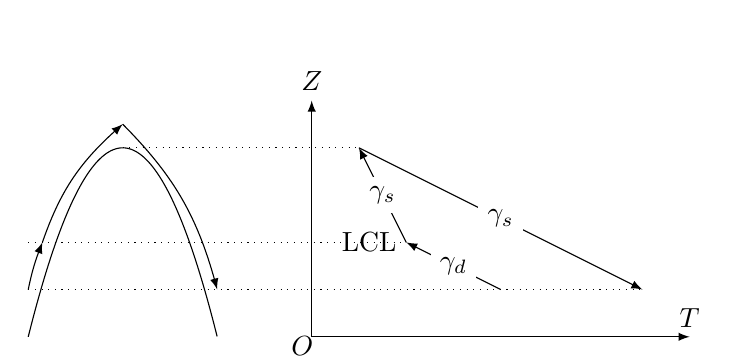
\begin{tikzpicture}[>=latex,scale=0.6]
        \draw [dotted](-2,1)--(11,1);
        \draw [dotted](-2,2)--(6,2);
        \draw [dotted](0,4)--(5,4);
        \draw [domain=-2:2,samples=1000]
        plot(\x,{-\x*\x+4});
        \draw[->](4,0)--(12,0)node[above]{\(T\)};
        \draw[->](4,0)--(4,5)node[above]{\(Z\)};
        \node at (3.8,-0.2){\(O\)};
        \draw[->](8,1)--node[fill=white]{\(\gamma_d\)}(6,2)node[left]{\(\mathrm{LCL}\)};
        \draw[->](6,2)--node[fill=white]{\(\gamma_s\)}(5,4);
        \draw[->](5,4)--node[fill=white]{\(\gamma_s\)}(11,1);
        \draw[->](-2,1) to [bend left=5](-1.7,2);
        \draw[->](-1.7,2) to [bend left=15](0,4.5);
        \draw[->](0,4.5) to [bend left=15](2,1);
    \end{tikzpicture}
    \caption{焚风}
\end{figure}

\section{温湿参量}

不同物理过程中基本变量所组合成一些特征量,并结合基本气象要素一起描述空气的状态,统称为温湿参量。

在干绝热过程中我们定义了位温,利用位温在干绝热过程中的保守性,比较两个干空气块的热力性质。

然而,位温在湿绝热过程中是增大的,不再具有保守性质。

所以,需要新建一个既考虑气压又考虑蒸发,凝结对气温影响的温湿特征量--相当位温。

湿绝热过程中的类似参量还有假相当位温和假相当温度,假湿球位温和假湿球温度等

\subsection{等压绝热过程--湿球温度}

系统:饱和湿空气+液态水

等压绝热过程为等焓过程

湿球温度,即在等压绝热蒸发过程中,系统内的液态水蒸发使气块降温,达到饱和时气块所具有的温度,是该过程中的最低温度。

实际工作中,湿球温度是用通风良好的湿球温度表直接测量的

这个热力学系统是由流经湿球的一定质量空气和从纱布蒸发出来的水分所组成的。

用实测湿球温度代替理论湿球温度,在通风良好的条伴下,其误差很小。

\subsection{等压绝热过程--相当温度}

相当温度或等压相当温度,定义为:系统经等压绝热蒸发过程成为湿空气以前,绝对干燥的空气所应具有的温度。是这个等压绝热蒸发过程中所可能有过的最高温度。

\subsection{假湿球位温和假湿球温度}

未饱和气块经过干绝热过程上升达到饱和后,再按照可逆饱和绝热过程下降到起始气压处的温度,称为假湿球温度,沿可逆饱和绝热过程下降到1000hPa处的温度,称为假湿球位温。
\begin{figure}[htbp]
    \centering
    \begin{tikzpicture}[>=latex]
        \draw[->](0,0)--(9,0)node[above]{\(T\)};
        \draw[->](0,0)--(0,5)node[above]{\(Z\)};
        \node at (-0.2,-0.2){\(O\)};
        \draw[dashed](4,1)--(2,3)node[below left]{\(\mathrm{LCL}\)}--node[below]{\(\gamma_s\)}(1,4)node[above]{\(B\)};
        \draw (6,1)--(2,3)node[above]{\(C\)};
        \draw (7,1)--node[fill=white]{\(\gamma_d\)}(1,4);
        \draw [dotted](0,3)node[above right]{\(p_c\)}--(2,3);
        \draw [dotted](0,1.8)node[above right]{\(p_0\)}--(3.2,1.8)node[above]{\(W\)}--(4.4,1.8)node[above]{\(A\)}--(5.4,1.8)node[above]{\(E\)};
        \draw [dotted](0,1)node[above right]{\(1000\mathrm{hPa}\)}--(7,1);
        \draw [dotted](2,0)node[below]{\(T_c\)}--(2,3);
        \draw [dotted](3.2,0)node[below]{\(T_{sw}\)}--(3.2,1.8);
        \draw [dotted](4,0)node[below]{\(\theta_{sw}\)}--(4,1);
        \draw [dotted](4.4,0)node[below]{\(T\)}--(4.4,1.8);
        \draw [dotted](5.4,0)node[below]{\(T_{se}\)}--(5.4,1.8);
        \draw [dotted](6,0)node[below]{\(\theta\)}--(6,1);
        \draw [dotted](7,0)node[below]{\(\theta_{se}\)}--(7,1);
    \end{tikzpicture}
    \caption{假湿球位温和假湿球温度}
\end{figure}

\(W\)点所对应的温度定义为假湿球温度,与前面所述的湿球温度十分相似,但又有所不同。\(T_w\)是等压绝热蒸发降温使气块达到饱和时的温度。\(T_{sw}\)虽然看起来也是绝热蒸发达到饱和时的温度,但其在上升和下沉的过程中多出一项对外做功。

通常\(T_w>T_{sw}\),但两者差异不大,一般不超过\(0.5^\circ\mathrm{C}\)。

另外,湿度越大,升降过程中气块对外做功也越小,两者差异也越小。

\subsection{假相当位温和假相当温度}

气块经过假绝热过程上升,直到全部水汽凝结脱落,然后再沿干绝热过程下沉到起始气高度处对应的温度为假相当温度\(T_{se}\),继续下沉到1000hPa对应的温度称作假相当位温\(\theta_{se}\)

注:假绝热过程可以看成是近似的等熵过程,故假相当位温也近似不变,是假绝热过程中的准保守量。

\section{混合过程}

\subsection{等压绝热混合}

等压绝热混合后系统的温度是混合前两气块各自初始温度的按质量加权平均。
\begin{equation}
T\approx\dfrac{m_1T_1+m_2T_2}{m}
\end{equation}

混合后的位温和水汽压的近似表达式:
\begin{equation}
\theta\approx\dfrac{m_1\theta_1+m_2\theta_2}{m}
\end{equation}

表明位温高的气块混合时位温下降,即气块放出热量,位温低的气块混合时位温上升,吸收热量,直到两个气块位温相等,热交换达到平衡为止。
\begin{equation}
e\approx\dfrac{m_1e_1+m_2e_2}{m}
\end{equation}

总之,两个未饱和气块绝热混合后,如无凝结发生,则终态的温度,水汽压取决于两个气块初态温度,水汽压的质量加权平均。

\subsection{垂直混合}

考虑两个不同高度的未饱和气块,垂直混合前,两个气块质量为\(m_1\)和\(m_2\),状态为(\(p_1,T_1,e_1\))和(\(p_2,T_2,e_2\))。

假设两气块先经过绝热过程移动到某一气层\(p(p_1>p>p_2)\),然后再做水平等压绝热混合,充分混合后变成一个质量为\(m=m_1+m_2\)的气块,其温度为\(T\),位温为\(\theta\),比湿为\(q\)。

\subsubsection{第一阶段}

气块按干绝热过程垂直移动到气层\(p\),但尚未混合。显然,此过程中,两个气块的\(q\)与\(\theta\)均不变,但\(T\)和\(e\)是变化的。则在气压\(p\)处时,有
\begin{gather}
    T'_1=T_1\left(\dfrac{p}{p_1}\right)^k=\theta_1\left(\dfrac{p}{1000}\right)^k\\
    T'_2=T_2\left(\dfrac{p}{p_2}\right)^k=\theta_2\left(\dfrac{p}{1000}\right)^k\\
    e'_1=e_1\dfrac{p}{p_1}\\
    e'_2=e_2\dfrac{p}{p_2}
\end{gather}

其中\(T'_1\)和\(T'_2\)分别表示两气块在同一高度处,混合前各自的温度,\(e'_1\)和\(e'_2\)分别为混合前各自的水汽压。

\subsubsection{第二阶段}

在气层\(p\)处,两个气块进行等压绝热混合,假设无凝结发生,则利用等压绝热混合方程
\begin{gather}
    q=\dfrac{m_1q_1+m_2q_2}{m}\\
    \theta\approx\dfrac{m_1\theta_1+m_2\theta_2}{m}\\
    T\approx\dfrac{m_1T'_1+m_2T'_2}{m}\\
    e\approx\dfrac{m_1e'_1+m_2e'_2}{m}
\end{gather}

根据以上公式,已知\(m_1,m_2,q_1,q_2,\theta_1,\theta_2\)的情况下,就计算出\(q,\theta,T,e\)等参量。

同样,也可求得\(T\)所对应的和水汽压\(e_s(T)\)。

如果\(e\leq{}e_s(T)\)那么在绝热混合过程中无凝结发生的假设成立,即这个混合后质量为\(m\)的气块内部不含液态水,

如果\(e\geq{}e_s(T)\)虽然无凝结发生的假设不成立,但混合后质量为\(m\)的气块内部发生的是等焓的不可逆凝结过程

因此可以按照假相当位温\(\theta_{se}\)近似不变的原理,得到有凝结情况下混合后气块的\(\theta_{se}\)为
\begin{equation}
\theta_{se}\approx\dfrac{m_1\theta'_{se1}+m_2\theta'_{se2}}{m}
\end{equation}

\chapter{热力学图像}

\section{大气热力学图}

热力图(Thermodynamic Diagram),能够描绘气压,温度和湿度的数值,并分析大气绝热过程和大气稳定度等。通常热力学图包含的线条有等压线,等温线,湿度线,干绝热线,饱和绝热(或假绝热)线。当气块经历一个绝热过程,其连续状态可以用图上的曲线表示,循环过程可以用一封闭曲线表示。一些图上的封闭曲线包围的面积与过程中环境对系统做的功成正比。

热力学图设计要素包括:
\begin{enumerate}
    \item 坐标为实测的气象要素,或其简单函数,纵坐标最好和高度成正比,
    \item 绘制的热力学线最好为直线,有利于绘图和分析,
    \item 等温线和绝热线的夹角尽可能大,这样热力过程图形随着随温度垂直梯度的变化就越敏感,
    \item 一些热力线就是气块状态变化曲线,
    \item 图上面积与能量成正比,便于计算大气运动能量,即为能量图解。
\end{enumerate}

\subsection{干绝热线}

埃玛图的等温线和干绝热线的夹角随位置而变,角度一般在\(45^\circ\)左右。等压线和等温线均为直线。在干绝热过程中,\(\theta\)为保守量。取一组不同的\(\theta\)值就能得到一组等温线,显然是一组对数曲线,由上可知,干绝热线为对数曲线,其斜率接近常数。

\subsection{等饱和比湿线}

等饱和比湿线是一组双曲线

埃玛图中等压面上的(绿色)短竖线为饱和虚温差,此处未画出。

\subsection{埃玛图示例}

埃玛图是一种能量图解,图上的面积表示了循环过程中外界对单位质量气块做功的大小。

在一个循环中,单位质量气块对外界做功为
\begin{equation}
w=R\oint{}T\mathrm{d}\ln(\dfrac{p_0}{p})=R\sigma'
\end{equation}

其中\(\sigma'\)为图中循环曲线所包围的面积,\(1\mathrm{cm}^2\)约等于\(74.5\mathrm{J\cdot{}kg^{-1}}\)

\subsection{大气层结曲线与状态曲线}

大气层结指一个地区上空大气温度和湿度的垂直分布。

探空资料中的温度,露点和压强的数值点绘在埃玛图上,用折线连接,层结曲线(\(p,T\))和露点层结曲线(\(p,T_d\))。

气块在此环境中做升降运动时,气块的温度和露点随气压而变化绘制于埃玛图上的曲线,称为气块的状态曲线。

\subsection{温湿参量的确定}
\begin{enumerate}
    \item 位温:状态点\(A(0,70)\)沿干绝热线下降(或上升)至1000hPa处所对应的温度。因干绝热线即等位温线,故而也可直接读取通过状态点\(A\)的干绝热线上的数值。
    \item 饱和比湿:读取通过状态点\(A\)的等饱和比湿线的数值,没有等饱和比湿线通过时,采用内插法求解,其结果即为状态点\(A\)的饱和比湿。
    \item 比湿:根据关系式\(q=\dfrac{\varepsilon{}e(T)}{p}=\dfrac{\varepsilon{}E_s(T_d)}{p}\)可知通过\(A'(p,T_d)\)点的饱和比湿即为实际比湿。
    \item 饱和水汽压:沿状态点\(A\)的等温线上升(\(T\)不变,则\(E_s\)不变),直到与\(p=622\mathrm{hPa}\)等压线相交于\(B\)点,通过\(B\)点的饱和比湿线的数值就是状态点\(A\)的饱和水汽压(\(E_s\))
    \item 实际水汽压:沿状态点\(A'\)的等露点温度线上升(\(T_d\)不变,则\(e\)不变),直到与\(p=622\mathrm{hPa}\)等压线相交与\(C\)点,通过\(C\)点的饱和比湿线的数值就是状态点\(A\)的实际水汽压(\(e\))。
    \item 抬升凝结高度:通过\(A'(p,T_d)\)的饱和比湿是状态点\(A\)的实际比湿,由\(A\)沿干绝热线上升,直到与通过\(A'\)的饱和比湿线相交,该交点即为凝结高度\(Z_c\)。
    \item 假相当位温:利用假相当位温的守恒性来求解。由于\(\theta{}_{se}\)在干湿绝热过程中守恒,湿绝热线就是等\(\theta{}_{se}\)线,因此只要读取通过抬升凝结高度\(Z_c\)点的湿绝热线上的\(\theta{}_{se}\)数值即可
\end{enumerate}

\begin{figure}[htbp]
    \centering
    \begin{minipage}{0.49\linewidth}
        \centering
        \caption{干绝热线}
        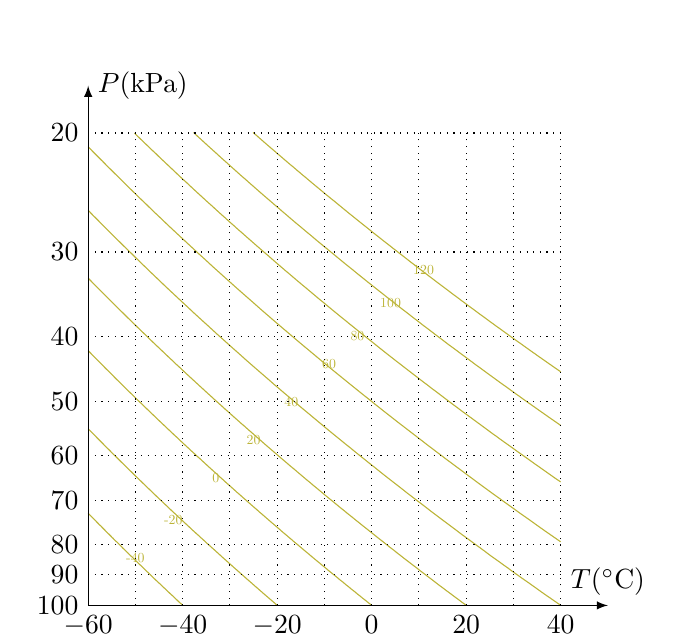
\begin{tikzpicture}[>=latex,scale=0.6]        
            \foreach \l in {-40,-20,...,40}
            {
                \draw [domain=0:{\l/10+6},color=yellow!70!black,samples=100]
                plot(\x,{(20-10*log10(100*pow((\x*10+213.15)/(\l+273.15),3.5)))*1.43});
            }
            \foreach \l/\d in {60/0,80/0.98,100/2.23,120/3.49}
            {
                \draw [domain={\d}:10,color=yellow!70!black,samples=100]
                plot(\x,{(20-10*log10(100*pow((\x*10+213.15)/(\l+273.15),3.5)))*1.43});
            }
            \foreach \t/\p in {1/\text{-40},1.8/\text{-20},2.7/\text{0},3.5/\text{20},4.3/\text{40},5.1/\text{60},5.7/\text{80},6.4/\text{100},7.1/\text{120}}
            {
                \node [color=yellow!70!black,scale=0.5]at(\t,\t){\p};
            }
            \draw[->](0,0)--(11,0)node[above]{\(T(\mathrm{^\circ{}C})\)};
            \draw[->](0,0)--(0,11)node[right]{\(P(\mathrm{kPa})\)};
            \foreach \x/\n in {0/\(-60\),2/\(-40\),4/\(-20\),6/\(0\),8/\(20\),10/\(40\)}
            {
                \draw [dotted] (\x,0) node[below]{\n} -- (\x,10);
            }
            \foreach \x in {1,3,...,9}
            {
                \draw [dotted] (\x,0) -- (\x,10);
            }
            \foreach \y/\m in {0/\(100\),0.65/\(90\),1.29/\(80\),2.22/\(70\),3.17/\(60\),4.31/\(50\),5.69/\(40\),7.48/\(30\),10/\(20\)}
            {
                \draw [dotted] (0,\y) node[left]{\m} -- (10,\y);
            }
        \end{tikzpicture}
    \end{minipage}
    \begin{minipage}{0.49\linewidth}
        \centering
        \caption{饱和比湿线}
        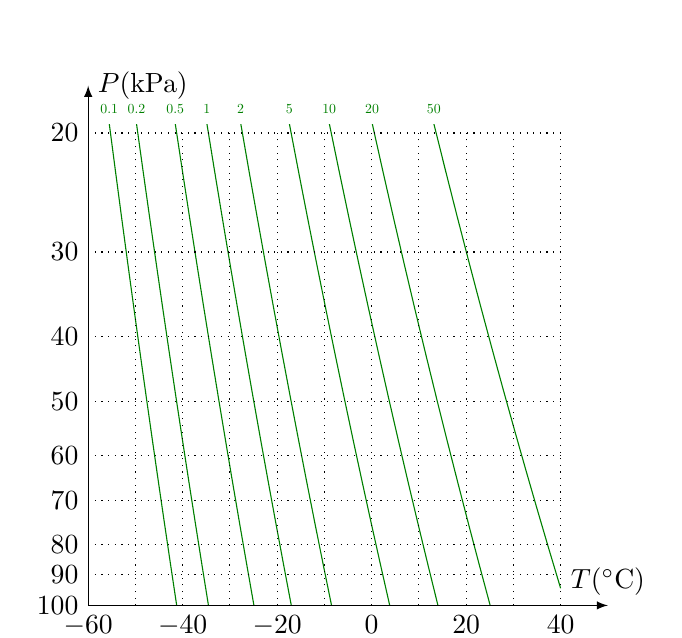
\begin{tikzpicture}[>=latex,scale=0.6]        
            \foreach \l/\a/\d in {0.1/0.445/1.873,0.2/1.021/2.545,0.5/1.842/3.509,1/2.513/4.3,2/3.228/5.15,5/4.258/6.383,10/5.102/7.403,20/6.01/8.51,50/7.317/10}
            {
                \node[color=green!50!black,scale=0.5] at (\a,10.5){\text{\l}};
                \draw [domain={\a}:{\d},samples=12,color=green!50!black]
                plot(\x,{(22.15-10*log10(622/\l+0.378)-75*(\x*10-60)/(177.3+10*\x))*1.43});
            }
            \draw[color=white] (0,10.2)--+(8,0);
            \draw[->](0,0)--(11,0)node[above]{\(T(\mathrm{^\circ{}C})\)};
            \draw[->](0,0)--(0,11)node[right]{\(P(\mathrm{kPa})\)};
            \foreach \x/\n in {0/\(-60\),2/\(-40\),4/\(-20\),6/\(0\),8/\(20\),10/\(40\)}
            {
                \draw [dotted] (\x,0) node[below]{\n} -- (\x,10);
            }
            \foreach \x in {1,3,...,9}
            {
                \draw [dotted] (\x,0) -- (\x,10);
            }
            \foreach \y/\m in {0/\(100\),0.65/\(90\),1.29/\(80\),2.22/\(70\),3.17/\(60\),4.31/\(50\),5.69/\(40\),7.48/\(30\),10/\(20\)}
            {
                \draw [dotted] (0,\y) node[left]{\m} -- (10,\y);
            }
        \end{tikzpicture}
    \end{minipage}\\
    \begin{minipage}{0.49\linewidth}
        \centering
        \caption{湿绝热线}%若能严格画出这条线请将此处图片替换,埃玛图中的湿绝热线已用注释符号包裹,不要忘记替换
        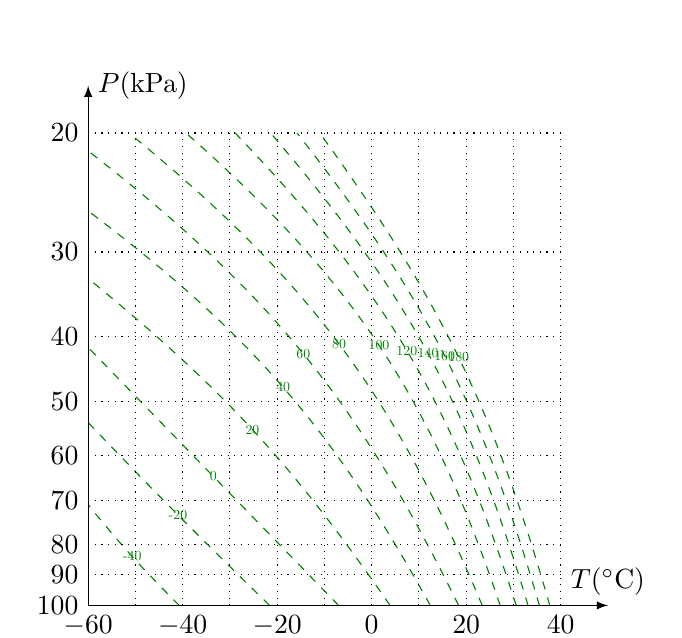
\begin{tikzpicture}[>=latex,scale=0.6]        
            \foreach \n/\x/\y/\b in {-40/1.93/2.13/-3,-20/3.84/3.87/-1,0/5.3/5.46/0,20/6.39/6.92/8,40/7.24/8.35/12,60/7.84/9.62/13}
            {
                \draw [dashed,color=green!50!black](\x,0) to [bend right=\b]node[scale=0.5]{\n}(0,\y);
            }
            \foreach \n/\p/\q/\b in {80/0.862/8.34/14,100/2.07/8.72/15,120/3.11/9.06/13,140/3.86/9.31/12,160/4.42/9.55/11,180/4.9/9.77/10}
            {
                \draw [dashed,color=green!50!black](\q,0) to [bend right=\b]node[scale=0.5]{\n}(\p,10);
            }
            \draw[->](0,0)--(11,0)node[above]{\(T(\mathrm{^\circ{}C})\)};
            \draw[->](0,0)--(0,11)node[right]{\(P(\mathrm{kPa})\)};
            \foreach \x/\n in {0/\(-60\),2/\(-40\),4/\(-20\),6/\(0\),8/\(20\),10/\(40\)}
            {
                \draw [dotted] (\x,0) node[below]{\n} -- (\x,10);
            }
            \foreach \x in {1,3,...,9}
            {
                \draw [dotted] (\x,0) -- (\x,10);
            }
            \foreach \y/\m in {0/\(100\),0.65/\(90\),1.29/\(80\),2.22/\(70\),3.17/\(60\),4.31/\(50\),5.69/\(40\),7.48/\(30\),10/\(20\)}
            {
                \draw [dotted] (0,\y) node[left]{\m} -- (10,\y);
            }
        \end{tikzpicture}        
    \end{minipage}
    \begin{minipage}{0.49\linewidth}
        \centering
        \caption{埃玛图}
        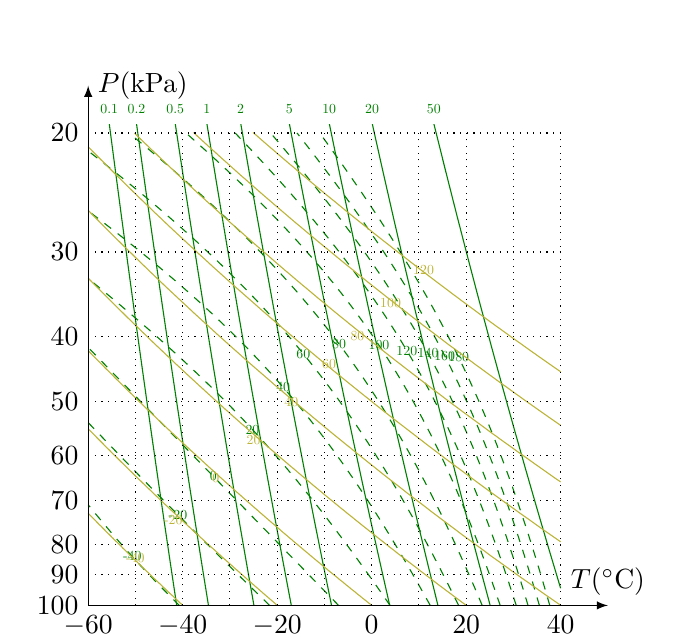
\begin{tikzpicture}[>=latex,scale=0.6]
            %%%%%%%%%%%%%%%%%%%%%%%%%%%%%%%%%%%%%%%%%%开始湿绝热线
            \foreach \n/\x/\y/\b in {-40/1.93/2.13/-3,-20/3.84/3.87/-1,0/5.3/5.46/0,20/6.39/6.92/8,40/7.24/8.35/12,60/7.84/9.62/13}
            {
                \draw [dashed,color=green!50!black](\x,0) to [bend right=\b]node[scale=0.5]{\n}(0,\y);
            }
            \foreach \n/\p/\q/\b in {80/0.862/8.34/14,100/2.07/8.72/15,120/3.11/9.06/13,140/3.86/9.31/12,160/4.42/9.55/11,180/4.9/9.77/10}
            {
                \draw [dashed,color=green!50!black](\q,0) to [bend right=\b]node[scale=0.5]{\n}(\p,10);
            }
            %%%%%%%%%%%%%%%%%%%%%%%%%%%%%%%%%%%%%%%%%%结束湿绝热线
            \foreach \l/\a/\d in {0.1/0.445/1.873,0.2/1.021/2.545,0.5/1.842/3.509,1/2.513/4.3,2/3.228/5.15,5/4.258/6.383,10/5.102/7.403,20/6.01/8.51,50/7.317/10}
            {
                \node[color=green!50!black,scale=0.5] at (\a,10.5){\text{\l}};
                \draw [domain={\a}:{\d},samples=12,color=green!50!black]
                plot(\x,{(22.15-10*log10(622/\l+0.378)-75*(\x*10-60)/(177.3+10*\x))*1.43});
            }
            \draw[color=white] (0,10.2)--+(8,0);
            \foreach \l in {-40,-20,...,40}
            {
                \draw [domain=0:{\l/10+6},color=yellow!70!black,samples=100]
                plot(\x,{(20-10*log10(100*pow((\x*10+213.15)/(\l+273.15),3.5)))*1.43});
            }
            \foreach \l/\d in {60/0,80/0.98,100/2.23,120/3.49}
            {
                \draw [domain={\d}:10,color=yellow!70!black,samples=100]
                plot(\x,{(20-10*log10(100*pow((\x*10+213.15)/(\l+273.15),3.5)))*1.43});
            }
            \foreach \t/\p in {1/\text{-40},1.8/\text{-20},2.7/\text{0},3.5/\text{20},4.3/\text{40},5.1/\text{60},5.7/\text{80},6.4/\text{100},7.1/\text{120}}
            {
                \node [color=yellow!70!black,scale=0.5]at(\t,\t){\p};
            }
            \draw[->](0,0)--(11,0)node[above]{\(T(\mathrm{^\circ{}C})\)};
            \draw[->](0,0)--(0,11)node[right]{\(P(\mathrm{kPa})\)};
            \foreach \x/\n in {0/\(-60\),2/\(-40\),4/\(-20\),6/\(0\),8/\(20\),10/\(40\)}
            {
                \draw [dotted] (\x,0) node[below]{\n} -- (\x,10);
            }
            \foreach \x in {1,3,...,9}
            {
                \draw [dotted] (\x,0) -- (\x,10);
            }
            \foreach \y/\m in {0/\(100\),0.65/\(90\),1.29/\(80\),2.22/\(70\),3.17/\(60\),4.31/\(50\),5.69/\(40\),7.48/\(30\),10/\(20\)}
            {
                \draw [dotted] (0,\y) node[left]{\m} -- (10,\y);
            }
        \end{tikzpicture}
    \end{minipage}\\
    \begin{minipage}{0.7\linewidth}
        \centering
        \caption{层结曲线与状态曲线}
        \begin{tikzpicture}[>=latex]
            \draw[->](0,0)--(8,0)node[above]{\(T\)};
            \draw[->](0,0)--(0,4.5)node[below right]{\(Z\)};
            \node at(-0.2,-0.2){\(O\)};
            \draw[->](7,0.5)--node[below]{\(\gamma_d\)}(4,1.5)node[left]{\(\mathrm{LCL}\)};
            \draw[->,dashed](4,1.5) to [bend right = 20](2,3.5);
            \draw(1,3.5) to [bend left = 10](7,0.5);
            \node at (5,2.5){层结曲线};
            \node at(3.5,2){\(\gamma_s\)};
            \node at(3,3.5){状态曲线};
        \end{tikzpicture}
    \end{minipage}
\end{figure}

\chapter{大气稳定}

\section{大气静力稳定度}

大气静力稳定度表示大气层结特性对气块铅直位移影响的趋势和程度。气象要素垂直分布,对流强弱,云雾降水形成,污染物扩散状况等,都与大气稳定度密切相关。

当大气处于静力平衡状态时,未饱和湿空气块受迫抬升后,可能出现三种情况

(1)稳定,(2)不稳定,(3)中性。

大气静力稳定度有以下特性:
\begin{enumerate}
    \item 静力稳定度是气块与它所的气层相互作用的综合结果
    \item 静力稳定度仅表示气块处在该气层中,其垂真运动发展的趋势与可能,
    \item 稳定气层中可以有对流运动,但不利于对流发展,不稳定气层中若无扰动也不可能发展对流,但有利于对流的发生,发展。
\end{enumerate}

\section{气块运动}

判断静力稳定度的方法通常使用气块法:理想气块在静力平衡的大气环境中受到扰动,根据气块的运动特征来判断大气稳定度的方法,在气块运动时,环境状态维持不变。

气块运动的趋势取决于气块与环境的热力差异,因气块运动中的热力状态是确定的,所以气块运动最终由环境大气的层结特征决定。

\section{气块法的假定条件}

在气层中的某一气块微团(服从气块假说)受到扰动而做绝热运动,但周围空气不受气块移动的影响,始终处于静力平衡状态。

气块是气层的一部分,其初始状态与同一高度上的其他大气相同,但它在假设静止不动的环境气层中做垂直运动时,就成了独立的部分。

气块在任何时刻都处于平衡态,状态方程和热一律均可适用。

\subsection{未饱和气块的大气层结稳定度}

对于未饱和气块,大气层结稳定度的性质取决于\(\Gamma-\gamma{}d\)
\begin{equation}
\begin{cases}
    \Gamma>\gamma{}d\quad\text{不稳定}\\
    \Gamma<\gamma{}d\quad\text{稳定}\\
    \Gamma=\gamma{}d\quad\text{中性}
\end{cases}
\end{equation}

也可用位温随高度的垂直变化率来表示大气层结稳定度。

根据公式\(\dfrac{\partial{}\theta}{\partial{}z}=\dfrac{\theta}{T}(\gamma{}_d-\Gamma)\),可知\(\dfrac{\partial{}\theta}{\partial{}z}\)与\(\gamma_d-\Gamma\)成正比,故有
\begin{equation}
\dfrac{\partial{}\theta}{\partial{}z}\begin{cases}
    <0\quad\text{不稳定}\\
    >0\quad\text{稳定}\\
    =0\quad\text{中性}
\end{cases}
\end{equation}

\subsection{饱和湿空气稳定度的判别}

与未饱和湿空气的方法类似,只要将\(\gamma_d\)换成\(\gamma_s\)即可。

因此饱和湿空气稳定度判据如下:
\begin{equation}
\Gamma\begin{cases}
    >0\quad\text{不稳定}\\
    <0\quad\text{稳定}\\
    =0\quad\text{中性}
\end{cases}
\end{equation}

同样也可由气层\(\theta{}_{se}\)随高度的变化率,得到与上式等价的判据
\begin{equation}
\dfrac{\partial{}\theta{}_{se}}{\partial{}z}\begin{cases}
    <0\quad\text{不稳定}\\
    >0\quad\text{稳定}\\
    =0\quad\text{中性}
\end{cases}
\end{equation}

如果薄气层的温度直减率\(\Gamma\)介于\(\gamma_d\)与\(\gamma_s\)之间,即\(\gamma_s<\Gamma<\gamma_d\)。那么
\begin{enumerate}
    \item 不含液态水的饱和薄汽层,它对扰动所产生的向上位移而言是不稳定的气层,对扰动所产生的向下位移而言是稳定的气层,
    \item 未饱和薄气层是稳定的,
    \item 未饱和薄气层是不稳定的,
\end{enumerate}

可见\(\gamma_s<\Gamma<\gamma_d\)的薄气层的静力稳定度视条件而定,称为条件性不稳定,这里的“条件性”是指气层是否饱和以及扰动产生位移的方向。

总结:大气静力稳定度的判据可以归纳为以下3种情形:
\begin{enumerate}
    \item \(\Gamma<\gamma_d\)(或\(\dfrac{\partial{}\theta}{\partial{}z}<0\))的薄气层,无论饱和或未饱和,该气层都是不稳定的,称为绝对不稳定的气层。
    \item \(\Gamma<\gamma_s\)(或\(\dfrac{\partial{}\theta_{se}}{\partial{}z}>0\))的薄气层,无论饱和或未饱和,该气层都是稳定的,称为绝对稳定的气层。
    \item \(\gamma_s<\Gamma<\gamma_d\)(或\(\dfrac{\partial{}\theta}{\partial{}z}>0\text{及}\dfrac{\partial{}\theta_{se}}{\partial{}z}<0\))的薄气层为条件性不稳定气层,若饱和且含液态水,则是不稳定的,若它是饱和但不含液态水,则受垂直向上扰动为不稳定,受垂直向下扰动就为稳定,如它未饱和,则为稳定。
\end{enumerate}

\section{不稳定能量}

\subsection{定义}

根据能量守恒和转化定律,如果环境大气对一上升气块做正功,那么气块垂直上升运动的动能是增加的,可以认为气块这种动能的增加是由气层所储藏的一部分能量转化而来的,这部分能量称为气层的不稳定能量。

根据定积分的几何意义,在埃玛图中,由气块状态曲线(虚线),大气层结曲线(实线)和等压线\(p_0\)--\(p\)所包围的面积,这个面积的大小与不稳定能量的多少成正比
\begin{figure}[htbp]
    \centering
    \begin{tikzpicture}[>=latex,scale=1]
        \draw[->](0,0)--(5,0)node[above]{\(T(\mathrm{^\circ{}C})\)};
        \draw[->](0,0)--(0,5)node[right]{\(\ln P(\mathrm{kPa})\)};
        \draw(1,1)node[left]{\(P_0\)}--(4,1);
        \draw[dotted](4,1)--node[right]{\(T_v\)}(3,4);
        \draw(3,4)--(1,4)node[left]{\(P\)};
        \draw(2,4)--(2.2,3)node[left]{\(T_{ve}\)}--(3,1.5)--(3.5,1);
        \node at(2.75,3){+};
        \node at(3.25,2){+};
        \node [scale=0.7]at(3,2.5){\(\Delta{}E>0\)};
    \end{tikzpicture}
    \caption{不稳定能量}
\end{figure}

\subsection{分类}
\subsubsection{潜在不稳定}
自由对流高度LFC,对流有效势能CAPE
\begin{equation}
\mathrm{CAPE}=R_d\int_{p_F}^{p_E}(T-T_e)\mathrm{d}(-\ln{}p)
\end{equation}

对流抑制能CIN
\begin{equation}
\mathrm{CIN}=-R_d\int_{p_1}^{p_F}(T-T_e)\mathrm{d}(-\ln{}p)
\end{equation}

\(E\)点为平衡高度,上拜加速度为0,垂直速度达到最大为
\begin{equation}
w_{max}=\sqrt{2\cdot{{}\mathrm{CAPE}}}
\end{equation}

\(w_{max}\)也是对流最终发展强弱的指标。
\begin{figure}[htbp]
    \centering
    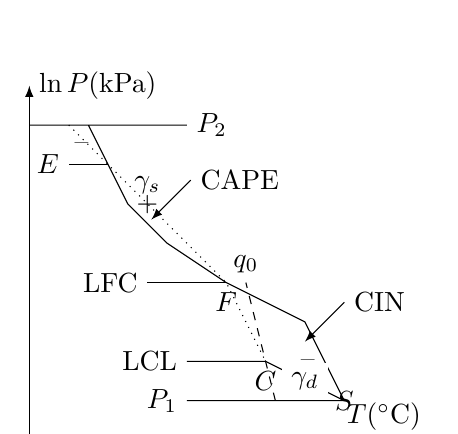
\begin{tikzpicture}[>=latex,scale=0.5]
        \draw[->](0,0)--(9,0)node[above]{\(T(\mathrm{^\circ{}C})\)};
        \draw[->](0,0)--(0,9)node[right]{\(\ln P(\mathrm{kPa})\)};
        \draw(4,1)node[left]{\(P_1\)}--(8,1)node{\(S\)}--node[left]{--}(7,3)--(5,4)node[below]{\(F\)}--(3.5,5)--node[above]{+}(2.5,6)--(2,7)--node[left]{--}(1.5,8)--(0,8)--(4,8)node[right]{\(P_2\)};
        \draw[dotted](1,8)--node[above]{\(\gamma_s\)}(5,4)--(6,2)node[below]{\(C\)};
        \draw[dashed](6.25,1)--(5.5,4)node[above]{\(q_0\)};
        \draw(8,1)--node[fill=white]{\(\gamma_d\)}(6,2)--(4,2)node[left]{LCL};
        \draw(5,4)--(3,4)node[left]{LFC};
        \draw(2,7)--(1,7)node[left]{\(E\)};
        \draw[->](4.1,6.6)node[right]{CAPE}--(3.1,5.6);
        \draw[->](8,3.5)node[right]{CIN}--(7,2.5);
    \end{tikzpicture}
    \caption{潜在不稳定}
\end{figure}

\subsubsection{绝对稳定}

如图所示,气块温度\(T\)总小于气层温度\(T_e\)。这种气层底部扰动不论强弱,气层对受扰气块起抑制作用,不利于受扰动气块的上升运动。

底部的气块并不是绝对不能上升。
\begin{figure}[htbp]
    \centering
    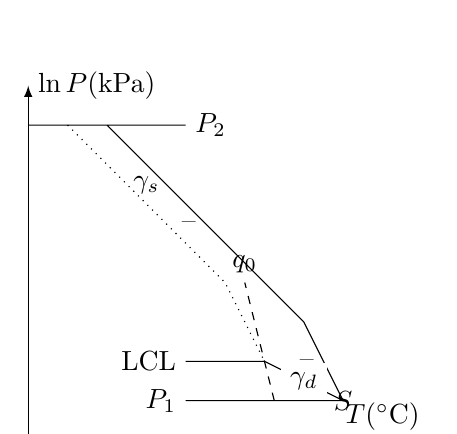
\begin{tikzpicture}[>=latex,scale=0.5]
        \draw[->](0,0)--(9,0)node[above]{\(T(\mathrm{^\circ{}C})\)};
        \draw[->](0,0)--(0,9)node[right]{\(\ln P(\mathrm{kPa})\)};
        \draw(4,1)node[left]{\(P_1\)}--(8,1)node{\(S\)}--node[left]{--}(7,3)--node[left]{--}(2,8)--(0,8)--(4,8)node[right]{\(P_2\)};
        \draw[dotted](1,8)--node[above]{\(\gamma_s\)}(5,4)--(6,2);
        \draw[dashed](6.25,1)--(5.5,4)node[above]{\(q_0\)};
        \draw(8,1)--node[fill=white]{\(\gamma_d\)}(6,2)--(4,2)node[left]{LCL};
    \end{tikzpicture}
    \caption{绝对稳定}
\end{figure}

\subsubsection{绝对不稳定}

如图所示,气块温度\(T\)总是大于气层温度\(T_e\)。

在这种气层中,低层大气是一个干绝热气层,其底部只要有一点微小的扰动,气块就能上升,该气层会释放不稳定能量并转化为气块上升的动能,使受扰动气块的上升运动得到发展。
\begin{figure}[htbp]
    \centering
    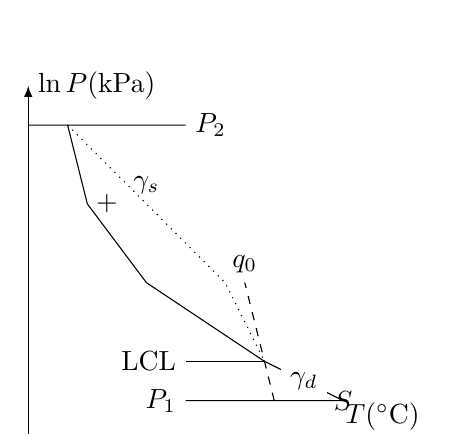
\begin{tikzpicture}[>=latex,scale=0.5]
        \draw[->](0,0)--(9,0)node[above]{\(T(\mathrm{^\circ{}C})\)};
        \draw[->](0,0)--(0,9)node[right]{\(\ln P(\mathrm{kPa})\)};
        \draw(4,1)node[left]{\(P_1\)}--(8,1)node{\(S\)}--node[fill=white]{\(\gamma_d\)}(6,2)--(3,4)--(1.5,6)--(1,8)--(0,8)--(4,8)node[right]{\(P_2\)};
        \draw[dotted](1,8)--node[above]{\(\gamma_s\)}(5,4)--(6,2);
        \draw[dashed](6.25,1)--(5.5,4)node[above]{\(q_0\)};
        \draw(6,2)--(4,2)node[left]{LCL};
        \node at (2,6){+};
    \end{tikzpicture}
    \caption{绝对不稳定}
\end{figure}

\chapter{辐射}

\section{辐射基本概念}

\subsection{特征}

任何物体,只要温度在绝对零度(0K)以上,都以电磁波形式向周围发射能量,同时又接收来自周围的电磁波。这种以电磁波形式传送能量的方式称为电磁辐射,其热交换形式称为辐射热交换。

电磁辐射的基本性质就是波粒二象性:即在经典电磁波理论中,能量的传播依靠电磁场的连续波动来完成,在量子理论中增加了辐射的粒子特征,物质发射或吸收的辐射能都以光子为单位。

辐射也表示电磁辐射通过真空传输的过程。真空中所有电磁波具有相同的传播速度,即光速
\begin{equation}
c=2.998\times10^8\mathrm{m\cdot{}s^{-1}}
\end{equation}

\subsection{物理量的关系}

当辐射在大气中传输时,因大气对辐射传输速度影响极小,所以依然认为辐射是以光速在传输。

电磁波的特性采用波长\(\lambda\),频率\(f\),波数\(\nu\),波速\(c\)和光子能量\(e\)来描述,它们之间的关系为
\begin{equation}
e=\dfrac{hc}{\lambda}\qquad\lambda\cdot{}f=c\qquad\nu=\dfrac{1}{\lambda}=\dfrac{f}{c}
\end{equation}

\(h\)为普朗克常数,\(h=6.626069934(89)\times10^{-34}\mathrm{J\cdot{}s}\)(NIST,2017)

波长:单位常用\(\mu{}\mathrm{m}(10^{-6}\mathrm{m})\),在UV和VIS波段也用\(\mathrm{nm}(10^{-9}\mathrm{m})\)。

波数:可以理解为“空间频率”,即单位长度内波动的个数,常用于在红外波段,单位是\(\mathrm{cm^{-1}}\)。

频率:的单位为Hz(赫兹),表示每秒振动次数。

电磁辐射具有不同的波长,按波长长短顺序排列而成的系列,称为电磁波谱。

太阳辐射能量主要集中在波长为0.1--4\(\mathrm{\mathrm{\mu{}m}}\)的区间,跨越了紫外线,可见光和近红外波段,也被称为短波辐射。

地球及其大气的热辐射主要位于4--120\(\mathrm{\mathrm{\mu{}m}}\)的谱段范围,属于红外波段,通常也被称为长波辐射。可见光,在整个电磁波谱中,可见光所占的波段其实很窄,大约为0.4--0.76\(\mathrm{\mathrm{\mu{}m}}\)。

\subsection{辐射的基本度量}
\begin{enumerate}
    \item 辐射能:以辐射形式通过空间某一表面传输的能量,以符号\(Q\)表示,单位J。
    \item 辐射通量:指单位时间内通过空间某一表面传输的辐射能,表示为\(\Phi=\dfrac{\mathrm{d}Q}{\mathrm{d}t}\),单位W。
\end{enumerate}

然而,描述辐射能量大小不仅涉及时间和空间上的分布,还需要考虑波谱和立体角上的分布。因为辐射能量的表示需要考虑单位立体角内的能量,所以这里先给出“立体角”的概念。

立体角定义为椎体所拦截的球面面积\(A\)与对应半径\(r\)平方之比,单位用球面度Sr表示,即
\begin{equation}
\Omega=\dfrac{A}{r^2}
\end{equation}

例如,上半球的立体角为:\(\Omega_{hemi}=\int_{0}^{2\pi}\int_{0}^{\frac{\pi}{2}}\sin{}\theta{}\mathrm{d}\theta\mathrm{d}\varphi=2\pi\)

\subsubsection{单色辐射亮度}

定义单色辐射亮度为:单位时间内,单位波长(即单位波谱区间内),在传播方向上的单位立体角内通过垂直于传播方向单位有效面积的辐射能量,通常用\(L_\lambda\),表示,定义式为:
\begin{equation}
L_\lambda=\dfrac{\mathrm{d}Q}{\mathrm{d}t\mathrm{d}\sigma'\mathrm{d}\Omega\mathrm{d}\lambda}
\end{equation}

单色辐射亮度也称为单色辐射强度,单位为\(\mathrm{J\cdot{}s^{-1}\cdot{}m^{-2}\cdot{}Sr^{-1}\cdot{}\mathrm{\mu{}m}^{-1}}\)。

注意:公式中的\(\mathrm{d}\sigma'=\cos{}\mathrm{d}\sigma\),即上式可改写为
\begin{equation}
L_\lambda=\dfrac{\mathrm{d}Q}{\cos{}\theta\mathrm{d}\sigma\mathrm{d}t\mathrm{d}\Omega\mathrm{d}\lambda}
\end{equation}

单色辐射强度实际上表示辐射场内任意位置,任意时刻,任意波长(或波数),沿任意方向传播的辐射的强弱程度。

也就是\(L_\lambda(x,y,z,t,\theta,\phi,\lambda)\),其中\((x,y,z)\)表示对应位置的面元面积,\(t\)表示对应时刻,\(\theta,\phi\)表示极坐标系下对应的方向,\(\lambda\)为对应波长。

单色辐射亮度是表征辐射场最基本的物理量,以它为基础,介绍单色辐射通量密度的概念,

单色辐射通量密度表示单位时间,单位波长通过单位面积的辐射能量,即沿不同方向传播的单色辐射亮度在平面法线方向的总和,通常用\(F\)表示,定义式为:
\begin{equation}
F_\lambda(x,y,z,t,\lambda)=\int_{2\pi}L_\lambda(x,y,z,t,\theta,\phi,\lambda)\cos{}\theta\mathrm{d}\Omega
\end{equation}

式中\(\cos\theta\)表示沿平面法向的分量,积分范围是平面上方整个半球\(2\pi\)球面度,\(F_\lambda\)单位为\(\mathrm{W\cdot{}m^{-2}\cdot\mathrm{\mu{}m}^{-1}}\)。普朗克定律由Max Planck于1900首次提出,描述了温度为\(T\),处于热平衡状态的绝对黑体发射辐射的规律,即其单色辐射强度\(B_\lambda(T)\)随波长的变化关系为:
\begin{equation}
B_\lambda(T)=\dfrac{2hc^2}{\lambda^5}\cdot\dfrac{1}{\mathrm{exp}\left(\dfrac{hc}{\lambda{}kT}\right)-1}
\end{equation}

黑体发射辐射的特点是辐射强度各向同性的,所以可利用朗伯定律得到黑体发射的单色辐射通量密度为:
\begin{equation}
F_{B,\lambda}(T)=\dfrac{2\pi{}hc^2}{\lambda^5}\cdot\dfrac{1}{\mathrm{exp}\left(\dfrac{hc}{\lambda{}kT}\right)-1}
\end{equation}

\subsubsection{物理意义}
\begin{enumerate}
    \item 黑体辐射与物质组成无关
    \item 黑体辐射强度随温度增高而增大
    \item 最大强度的波长随温度增高而减小
\end{enumerate}

\subsubsection{总结}

绝对黑体,它的发射辐射只取决于温度,与物体的形状和成分无关。同时,由光谱辐射强度可以反推出对应波长上发射出等量辐射的黑体温度,该温度通常被称为亮度温度(或等效黑体温度)。

当辐射波长向两端变化,波长趋于无穷大或无限接近零时,普朗克函数的极限可以分别得到\(\lambda\rightarrow\infty\)时的瑞利--金斯分布和\(\lambda\rightarrow{}0\)时的维恩分布。黑体辐射光谱最大值对应波长\(\lambda\)与温度\(T\)反比的关系,该规律被称为维恩定律或维恩位移定律。

最大波长和黑体温度是一一对应的,所以可以根据这个辐射最强的波长确定绝对黑体的温度,这个温度被称为颜色温度或色温,而这就是光谱法测量物体温度的基础。

绝对黑体发射的总辐射能量和温度的4次方成正比,这一规律被称为斯蒂芬--玻尔兹曼定律。利用斯蒂芬--玻兹曼定律得到对应绝对黑体的温度,该温度被称为有效温度(不局限于黑体)。

在辐射平衡条件下,任何物体的单色辐射通量密度\(F_{\lambda,T}\),与吸收系数\(A_{\lambda,T}\)成正比关系,二者比值只是波长和温度的函数,与物体性质无关。任何物体的辐出度和它的吸收率之比都等于同一温度下黑体的辐出度\(F_B\)
\begin{equation}
\dfrac{F_{\lambda,T}}{A_{\lambda,T}}=F_{B(\lambda,T)}
\end{equation}

若定义比辐射率\(\epsilon _{\lambda,T}\)为物体的放射能力\(F_{\lambda,T}\)和黑体的辐射能力\(F_{B(\lambda,T)}\)之比,则基尔霍夫定律可以写成
\begin{equation}
\epsilon _{\lambda,T}=A_{\lambda,T}
\end{equation}

意义:将物体的吸收能力和放射能力联系起来,将各种物质的吸收,放射能力与黑体的吸收放射能力联系起来。

\section{大气对辐射的吸收}

\subsection{吸收情况}

辐射通过介质时,一部分能量被介质吸收而转化为热能或者内能,并且深入介质越深,强度就衰减越大,这就是介质对辐射的吸收现象。

对于波长小于\(0.29\mathrm{\mathrm{\mu{}m}}\)的太阳辐射,吸收率接近1。\(\mathrm{O}_2,\mathrm{O}_3\)把\(0.29\mathrm{\mathrm{\mu{}m}}\)以下的紫外辐射几乎全部吸收,可见光波段只有非常少量的吸收,红外波段主要是水汽的吸收,其次是\(\mathrm{CO}_2\)和\(\mathrm{CH}_4\)。\(14\mathrm{\mathrm{\mu{}m}}\)以外的辐射不能透过大气传向外太空。

\subsection{重要的窗区}

可见光窗区:0.4--0.76\(\mathrm{\mathrm{\mu{}m}}\)

大气透明窗或大气光谱窗:8--12\(\mathrm{\mathrm{\mu{}m}}\)大气的吸收很弱

地表的温度约300K,与这个温度相对应的黑体辐射能量主要集中在10\(\mathrm{\mathrm{\mu{}m}}\)这一范围,通过窗区,地面发出的长波辐射可顺利地被发送到宇宙空间。

大气窗区对地气平衡有十分重要的意义。

\subsection{大气对辐射的吸收与散射}

\subsubsection{吸收}

吸收截面\(\sigma_a\):粒子所吸收的辐射通量相当于面积\(\sigma_a\)从入射辐射场中所截获的辐射通量。

体积吸收系数:单位体积中各粒子吸收截面之和:\(k_a=N\cdot\sigma_a\)。(单位\(\mathrm{m}^2\cdot\mathrm{m}^{-3}\)或\(\mathrm{m}^{-1}\))

质量吸收系数:单位质量中各粒子吸收截面之和,单位质量的吸收物质(\(1\mathrm{cm}^2\)气柱中)吸收了原辐射能的份数:
\begin{equation}
\rho\cdot{}k'_a=k_a\quad{}k_{ab}=N\sigma_{ab}=\sigma_{ab}\dfrac{N_0}{M}\rho=k'_{ab}\rho
\end{equation}

\subsubsection{散射}

大气对辐射的散射:气体分子以及气溶胶粒子内答有多个分立的电子和质子,当电磁波照射到粒子上后,使正负电荷中心产生偏移,构成电偶极子或多极子,并在电磁波激发下做受迫振动,向各方向发射次生电磁波。这种次生电磁波就散射辐射。

特点:散射波长和原始波相同并,与原始波有固定的位相关系。

\subsubsection{区别}

散射不产生分子内能状态的变化,应以电磁波理论和物质的电子理论来解释(米理论),吸收是因能态发生变化而产生的,需要用量子理论来解释。

散射不是选择性的,它在电磁波谱的各个波长上都会发生,因而是全波段的

\subsection{无量纲数}

定义无量纲尺度参数\(\alpha=\dfrac{2\pi{}r}{\lambda}\)
\begin{enumerate}
    \item 当\(\alpha<<1(r<\lambda)\):Rayleigh散射,也称分子散射,如空气分子对短波辐射的散射。
    \item 当\(0.1<\alpha<50(r\approx\lambda)\):Mie散射,如大气中的云滴等气溶胶粒子对短波辐射的散射。
    \item 当\(\alpha>50(r\geq\lambda)\):几何光学散射范畴。如大雨滴对可见光的折射,反射。
\end{enumerate}

瑞利散射削弱系数与波长的4次方成反比,波长越短,分子散射削弱越强。

米散射理论是球状粒子散射的通用理论

\subsection{辐射能在吸收介质中的传输}

指数削弱规律:比尔(Beer)定律设有单色平行定向辐射束的辐照度为\(E_\lambda\),经过气层\(\mathrm{d}l\)后
\begin{equation}
\mathrm{d}E_\lambda=-E_\lambda\cdot\sigma_{a,\lambda}N\mathrm{d}l=-E_\lambda\cdot{}k_{a,\lambda}\mathrm{d}l
\end{equation}

质量吸收系数表示
\begin{equation}
\mathrm{d}E_\lambda=-E_\lambda\cdot\rho{}k'_{a,\lambda}\mathrm{d}l
\end{equation}

光学厚度:沿辐射传输路径,单位截面上所有吸收和散射物质产生的总削弱
\begin{equation}
\delta_\lambda=\int_0^lk_{ex,\lambda}\mathrm{d}l=\int_{0}^{l}\rho\cdot{}k'_{ex,\lambda}\mathrm{d}l
\end{equation}

则比尔定律可写为
\begin{equation}
E_{\lambda,l}=E_{\lambda,0}\cdot{}\mathrm{exp}(-\delta_\lambda)
\end{equation}

整层大气垂直光学厚度定义为:
\begin{equation}
\delta_\lambda(0)=\int_{0}^{\infty}k_{ex,\lambda}(z)\mathrm{d}z=\int_{0}^{\infty}\rho\cdot{}k'_{ex,\lambda}(z)\mathrm{d}z
\end{equation}

光学质量:辐射束沿传输路径在单位截面气柱内所含吸收或散射气体的质量。
\begin{equation}
u=\int_{0}^{l}\rho\mathrm{d}l
\end{equation}

太阳常数:在大气上界日地平均距离处,通过与太阳光垂直的单位面积上,单位时间接收的能量(即积分辐照度)。以符号\(\bar{S}_0\)表示为
\begin{equation}
\bar{S}_0=\int_{0}^{\infty}S_\lambda\mathrm{d}\lambda
\end{equation}

其中\(S_\lambda\),为在日地平均均距离\(d_0\)处大气上界,与日光垂直平面上的太阳分光辐照度。

太阳常数数值范围在1339~1396\(\mathrm{W\cdot{}m}^2\)

\subsection{定位坐标}
\begin{enumerate}
    \item 天顶角zenith(ZEN):太阳方向与垂直法向夹角。
    \item 高度角altitude(ALT)=\(90^\circ-\)ZEN:太阳方向与水平面夹角。
    \item 方位角azimuth(AZI):一般是以观测点的正北方向为起始方向,以太阳光的入射方向为终止方向,按顺时针方向所测量的角度。AZI通常以正北方向为零,按顺时针方向增大变化,范围在\(0^\circ\)--\(360^\circ\)。正北AZI=\(0^\circ\),正东AZI=\(90^\circ\),正南AZI=\(180^\circ\),正西AZI=\(270^\circ\)。
    \item 时角hour angle(HRA):观测点的经圈与太阳重合后(即当地正午)地球自转的角距离。由于地球的自转,太阳时角每小时增长\(15^\circ\),所以时角常用相应的时间单位,以0--24h取代\(0^\circ\)--\(360^\circ\)。
\end{enumerate}

太阳天顶角计算

某一时刻观测到的太阳天顶角\(\theta\)的计算公式为
\begin{equation}
\cos{}\theta=\sin{}\phi\sin{}\delta+\cos{}\phi\cos{}\delta\cos{}h
\end{equation}

太阳高度角为天顶角的余角。

太阳方位角计算。
\begin{equation}
\cos{}\alpha=\dfrac{\sin{}\delta-\sin{}\phi\cdot\cos{}\theta}{\cos{}\phi\cdot\sin{}\theta}
\end{equation}

在日出日落时刻,天顶角90°可得日出,日落时的太阳方位角和时角分别为
\begin{gather}
    \cos{}\alpha_0=\dfrac{\sin{}\delta}{\cos{}\phi}\\
    \cos{}h_0=-\dfrac{\tan{}\delta}{\tan{}\phi}
\end{gather}

\(\alpha_0\)和\(h\)随地点\(\Phi\)和季节\(\delta\)而不同。

例如对北半球的春(秋)分日,\(\delta=0,h_0=\pm\pi/2,\alpha_0=90^\circ\text{和}270^\circ\),即日夜等长,太阳从正东方升起,从正西方落下,夏至日\(\delta=23.5^\circ\),在\(\Phi=66.5^\circ\)处,\(h_0=\pm{}\pi\),说明北极圈内全天太阳不落。

\section{辐射路径}

到达地面的太阳总辐射包括两部分:直接辐射和散射辐射。

\subsection{直接辐射由太阳天顶角\(\theta\)和光学厚度决定。}

太阳辐射在大气中的散射,一部分通过后向散射向上辐出大气层,另一部分通过前向散射到达地面。组成云的水滴和冰晶是强烈的散射体和吸收体,因此云对太阳辐射的调节起着重要作用。

\subsection{云的吸收作用}

云吸收太阳辐射的多少,主要由云的光学厚度,单次散射比和散射相函数决定。通常云越厚,云滴尺度越大,其吸收越强。当云厚度超过500m时,吸收率近似为常数。此外,云的吸收率随太阳高度角的增大而增大。

云对太阳辐射的吸收作用小于云的散射作用。

\subsection{云的反射作用}

由于云中水滴和冰晶的散射,使云体表面称为强大的反射面,将部分入射太阳辐射反射回太空,对其下大气和地面起到冷却作用。

到达地面的太阳总辐射等于直接辐射和散射辐射之和。

\subsection{长波辐射在大气传输过程中的特点}
\begin{enumerate}
    \item 地球和大气都是放射红外辐射的辐射源,通过大气中的任一平面射出的是具有各个方向的漫射辐射。
    \item 除非在大颗粒物质较多时,大气对长波辐射的散射削弱极小,可以忽略不计,因此研究长波辐射时,通常只考虑吸收作用。
    \item 大气不仅是削弱辐射的介质,而且还同时放射长波辐射,有时其放射的辐射甚至会超过吸收部分,所以必须将大气的放射与吸收同时考虑。
    \item 总之,长波辐射在大气中的传输是一种漫射辐射,是在无散射但既有吸收又有放射的质中的传输。
\end{enumerate}

\section{大气模型}


若将整个地气系统视为一个黑体,则吸收速率=发射速率

收入:\(\bar{S}_0\cdot\pi{}R_E(1-a_E)\)

支出:\(4\pi{}R_E^2\cdot\sigma{}T_E^4\)

若取:\(\bar{S}_0=1366\mathrm{W\cdot{}m}^{-2},a_E=0.3\),则\(T_E=255\mathrm{K}\)
\begin{equation}
\dfrac{\bar{S}_0}{4}(1-a)\approx239.4\mathrm{W\cdot{}m}^{-2}
\end{equation}

地球表面收到的太阳辐射平均辐照度也是地球发射的长波平均辐出度

地--气系统的两个组成部分是地球和大气。它们对辐射的吸收和发射的特性不同。

大气对短波辐射吸收比较小,而对长波辐射有一定的吸收和发射。

\subsection{单层大气}
\begin{table}[htbp]
    \centering
    \begin{tabular}{cc|cc}
        \multicolumn{2}{c|}{短波辐射}&\multicolumn{2}{c}{长波辐射}\\
        \(\downarrow \dfrac{\bar{S}_0}{4}\)&\(\uparrow \dfrac{\bar{S}_0}{4}a_E\)&\(\uparrow A_L\sigma{}T_a^4\)&\(\uparrow (1-A_L)\sigma{}T_a^4\)\\
        \hline
        \multicolumn{2}{c|}{大气}&\multicolumn{2}{c}{大气}\\
        \hline
        \multicolumn{2}{c|}{\(\downarrow \dfrac{\bar{S}_0}{4}\)}&\(\downarrow A_L\sigma{}T_a^4\)&\(\uparrow F_2\sigma{}T_a^4\)\\
        \hline
        \hline
    \end{tabular}
    \caption{单层大气}
\end{table}

则地面和大气顶的辐射平衡方程为
\begin{equation}
\begin{cases}
    \dfrac{\bar{S}_0}{4}-\dfrac{\bar{S}_0}{4}a_E-A_L\sigma{}T_a^4-(1-A_L)\sigma{}T_g^4=0\\
    \bar{S}_0(1-a_E-A_s)+A_L\sigma{}T_a^4-\sigma{}T_g^a=0
\end{cases}
\end{equation}

单层大气辐射平衡的解
\begin{gather}
    T_g^4=\dfrac{\bar{S}_0}{4}\cdot\dfrac{2(1-a_E)-A_s}{\sigma(2-A_L)}\\
    T_a^4=\dfrac{\bar{S}_0}{4}\cdot\dfrac{A_s-A_L(1-a_E-A_s)}{\sigma{}A_L(2-A_L)}
\end{gather}

若设\(A_L=0.8,A_s=0.2,a_E=0.3\)可得
\begin{equation}
T_g=278.6\mathrm{K},T_a=247.7\mathrm{K}
\end{equation}

大气层的平均温度低于全球的有效温度。当\(A_L\),增大时,地面平均温度也将升高。

\subsection{二层大气模型}
\begin{table}[htbp]
    \centering
    \begin{tabular}{cccc}
        \(\downarrow E\)&\(\uparrow F_g(1-A)^2\)&\(\uparrow F_1(1-A)\)&\(\uparrow F_2\)\\
        \hline
        \multicolumn{4}{c}{上层大气}\\
        \hline
        \(\downarrow E\)&\(\uparrow F_g(1-A)\)&\(\uparrow F_1\)&\(\downarrow F_2\)\\
        \hline
        \multicolumn{4}{c}{下层大气}\\
        \hline
        \(\downarrow E\)&\(\uparrow F_g\)&\(\downarrow F_1\)&\(\downarrow F_2(1-A)\)\\
        \hline
        \hline
    \end{tabular}
    \caption{二层大气模型}
\end{table}

辐射平衡方程
\begin{equation}
\begin{cases}
    E=0.25F_g+0.5F_1+F_2\\
    E=0.5F_g+F_1-F_2\\
    E=F_g-F_1-0.5F_2
\end{cases}
\rightarrow
\begin{cases}
    F_2=E/3\\
    F_1=E/2\\
    F_g=5E/2
\end{cases}
\end{equation}

其中\(F_g=\sigma{}T_g^4,F_1=A\sigma{}_{a_1}^4,F_2=A\sigma{}_{a_2}^4\)
\begin{gather}
    T_{a_2}=(0.33E/0.5\sigma)^{1/4}=231\mathrm{K}\\
    T_{a_1}=(0.5E/0.5\sigma)^{1/4}=255\mathrm{K}\\
    T_{g}=(1.67E/0.5\sigma)^{1/4}=290\mathrm{K}
\end{gather}

\section{地气系统的净辐射}
系统或物体收入辐射能与支出辐射能的差值称为净辐射,也称辐射差额。

例如,对于净辐射通量密度\(F^*\),它是收入辐射通量密度\(F_i\),与支出辐射通量密度\(F_o\)的差
\begin{equation}
F^*=F_i-F_o
\end{equation}

入射到地面的长波辐射来自整层大气的辐射,称为大气逆辐射,它取决于大气层温度与湿度的垂直分布,且和云的状况有密切关系,但没有显著的日变化。

大气逆辐射由两部分组成:
\begin{enumerate}
    \item 来自大气本身的热辐射,主要是1--2km内的\(\mathrm{H_2O}\)和\(\mathrm{CO_2}\)的发射,
    \item 云的热辐射,由云体发出并经过大气窗区达到地面的长波辐射。
\end{enumerate}

地面向上的长波辐射包括地面发射的长波辐射和地面反射的部分大气逆辐射

地面有效辐射=地面向上长波辐射-大气逆辐射

晴朗干燥夜晚,地面有效辐射大,地面降温明显,有云时,大气逆辐射增强,使地面有效辐射减小,特别是有低云且云量大时,地面有效辐射可能只有无云时的1/4。

\end{document}